\documentclass{article}

\usepackage[a4paper, total={6in, 8in}]{geometry}
\usepackage[utf8]{inputenc}
\usepackage{fancyhdr}
\usepackage{graphicx}
\usepackage{enumitem}

\pagestyle{fancy}
\fancyhf{}
\lhead{John J Li}
\rhead{CSE360 Summer 2021 Notes}
\rfoot{\thepage}
\renewcommand{\headrulewidth}{0.4pt}

\setlength{\parskip}{1em}
\setlength\parindent{0px}
\title{CSE360 Summer 2021 Notes}
\date{\today}
\author{John J Li}

\begin{document}
    \maketitle
    \thispagestyle{empty}
    \noindent\rule{\textwidth}{0.8pt}

    \section*{Plan-driven Process Models}

    A plan-driven model plans process activities in advance and the progress is 
    measured against the plan.
    There are 5 types of plan-driven models: waterfall, v-model, incremental, prototype,
    and spiral.

    \subsection*{Waterfall Model}

    Each fundamental process activity is placed into seperated phases and performed in a
    linear order.
    Use this when requirements are well understood and won't likely change, it is a 
    large system, and multiple companies are involved. Commonly used in financial, security,
    gov/military, embedded systems. Difficult to change once the process starts.

    \begin{center}
        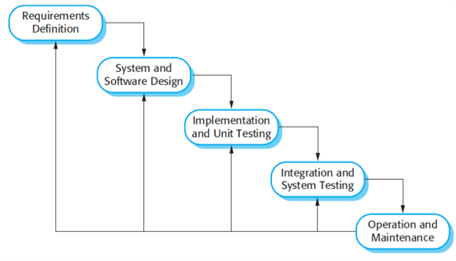
\includegraphics[scale=0.7]{WaterfallModel.png}
    \end{center}

    \subsection*{V-Model}

    Extension of waterfall model -- process steps are bent upwards after the coding phase.
    Each dev phase has a testing phase.
    Verification (leftside) analyzes that the requirements are met. Validation (right side)
    tests that the implementation meets the requirements.
    Useful for maintaining strict deadlines and milestones and detecting errors earlier in
    the dev process.

    Unit testing eleminates bugs at code or unit level. Integration testing verifies 
    communication between modules. System testing tests the complete application 
    and function and non-function requirements. User acceptance testing 
    verifies applicaiton is ready for the real world.

    \begin{center}
        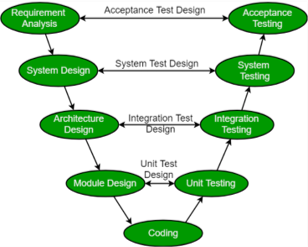
\includegraphics[scale=0.7]{V-Model.png}
    \end{center}

    \subsection*{Incremental Model}

    Split activities into pieces. It is an iterative model. Develop an initial implementation
    which complete a portion of each activity and gets user feedback then evolve the next 
    implementation version and repeat.

    There is frequent user feedback and reduce cost of changing requirements plus a 
    rapid delivery of useful software.
    However it is harder to measure progress and system structure tends to degrade 
    as new increments are added.

    \begin{center}
        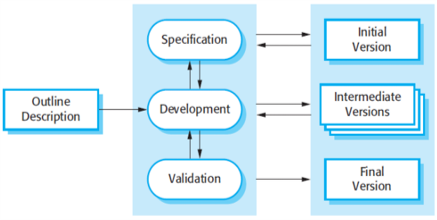
\includegraphics[scale=0.7]{IncrementalModel.png}
    \end{center}

    \subsection*{Prototyping}

    Early version of the system or part of the system that is developed quickly. 
    Customers are involved through this process and it anttcipate changes but is often 
    discarded.

    \begin{center}
        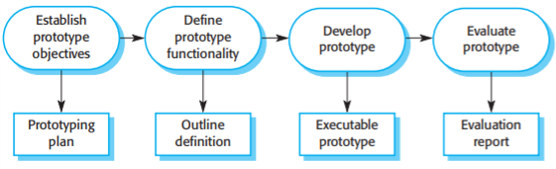
\includegraphics[scale=0.7]{Prototyping.png}
    \end{center}

    \subsection*{Spiral Model}

    Similar to the incremental model, but includes risk assessment. Each loop represents a 
    phase. Determine goals in top left, evaluate risks in top right, develop and test in 
    bottom right, and plan in bottom left.

    This is useful for large projects, high-risk projects, needing a lot of documentation,
    and there are significant changes are expected. Doesn't work for small projects, project 
    time estimation is difficult and success is dependent on effective risk assessment.

    \begin{center}
        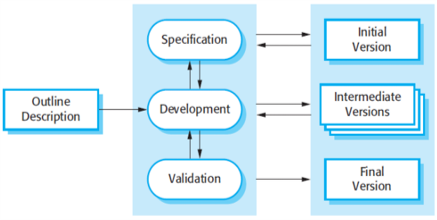
\includegraphics[scale=0.7]{IncrementalModel.png}
    \end{center}

    \section*{Agile Process Models}

    The agile model plans in increments and can change to reflect changes in requirements.
    There are 2 types of agile models: SCRUM and XP(extreme programming). Emerged in the 
    1980s and 1990s focused on code and an iterative approach to software development.
    The aim was the reduce overheads in the software process by limiting documentation 
    and responding quickly to changes.

    \subsection*{Manifesto for Agil Software Development}

    “We are uncovering better ways of developing software by doing it and helping others 
    do it. Through this work, we have come to value:

    \begin{itemize}
        \item Individuals and interations over processes and tools
        \item Working software over comprehensive documentation
        \item Customer collaboration over contract negotiation
        \item Responding to change over following a plan
    \end{itemize}

    That is, while there is value in the items on the right, we value the item on the left 
    more.”

    \subsection*{Agile Definition}

    \begin{itemize}
        \item Software development under which requirements and solutions evolve through 
        the collaborative effort of self-organizing cross-functional teams
        \item
        Adaptive planning to provide a rapid and flexible response to change
        \item
        Incremental lightweight process
        \item
        Early delivery
        \item
        Feedback-driven empirical approach
    \end{itemize}

    \subsection*{Extreme Programming (XP)}

    Several new versions may be developed by different programmers at the same time.
    They write tests for each task before writing code. This is difficult to integrate with 
    typical business practices. Requirements expressed as user stories.

    \subsection*{User Scenarios and User Stories}

    User Scenario: Long description for the user of the product. Can include mulitple 
    requirements.
    User Story: Short description of one requirement such as "As a <user>, I want <feature>
    so I can <rationale>.

    \subsection*{Agile vs Plan-driven Dev}

    Plan-driven
    \begin{itemize}
        \item 
        Each phase requires formal documentation (i.e. requirements specification) between 
        each major process activity, i.e.
        \item
        Requirements engineering: identify all requirements
        \item
        Requirements specification: document requirements
        \item
        Design and implementation: determine how to satisfy requirements and implement it
    \end{itemize}
    Agile
    \begin{itemize}
        \item 
        Each iteration goes through all the activities
        \item
        Often requirements and design are developed together rather than separately
    \end{itemize}

    \begin{center}
        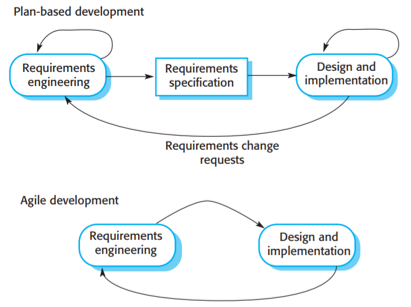
\includegraphics[scale=0.7]{AgileVSPlan.png}
    \end{center}

    \subsection*{Scrum}

    There is the product owner which communicate vision of the product to the dev team 
    and they represents customer's interests. There is the scrum master who is the 
    leader in the team and acts between product owner and team. Finally, there is the 
    individual team members.

    First there is the product backlog which prioritizes list of items that need to be
    worked on. Then comes sprint backlog which is the set of features that will 
    be worked on in the upcoming sprint. Then the sprint which is the time period to
    develop the next iteration and includes a daily scrum meeting which is a meeting to 
    ask about progress and issues.

    \begin{center}
        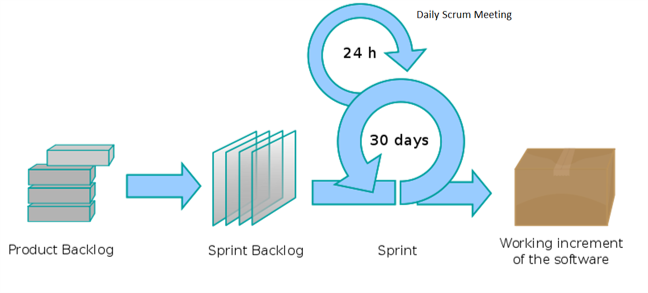
\includegraphics[scale=0.6]{Scrum.png}
    \end{center}

    \subsection*{Agile Benefits}

    \begin{itemize}
        \item 
        Product is broken down into a set of manageable and understandable chunks
        \item
        Unstable requirements do not hold up progress
        \item
        The whole team can see what is happening at every step and leads to improving team communication
        \item
        Customers see on-time delivery of increments and can get feedback on how well the product works
        \item
        Works well on small to medium-sized products
    \end{itemize}

    \subsection*{Agile Challenges}

    \begin{itemize}
        \item 
        The informality of agile development is incompatible with the legal approach to contract definition (requirement specification) that is commonly used in large companies
        \item
        Agile methods are most appropriate for new software development rather than software maintenance
        In large companies, a lot of work is devoted to maintaining existing software systems
        \item
        Agile methods are designed for small co-located team, yet software development now involves worldwide, distributed teams
    \end{itemize}

    \section*{Requirements Engineering}

    \subsection*{Types of Requirements}

    User requirements
    \begin{itemize}
        \item 
        Statements are written in the natural language
        \item
        Diagrams of the services the system provides and its operational constraints
        \item
        Varies between broad statements of system features to detailed, precise descriptions of system functionality
        \item
        Typically, written for customers
    \end{itemize}

    System requirements
    \begin{itemize}
        \item 
        Structured document setting out detailed descriptions of the system’s functions, services, and operational constraints
        \item
        Defines exactly what is to be implemented
        \item
        Typically, written for developers
    \end{itemize}

    \begin{center}
        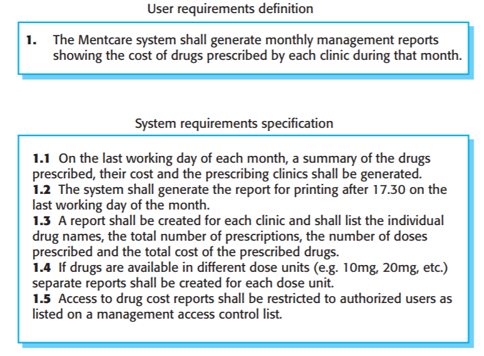
\includegraphics[scale=0.7]{types_of_requirements.png}
    \end{center}

    \subsection*{Functional Requirements}

    Statements of services the system should provide.
    How should the system react to particular inputs?
    How should the system behave in particular situations?
    May state what the system should not do.
    And is typically written in natural language.

    \subsection*{Non-functional Requirements}

    Requirements are not directly related to specific services and often applies to the 
    system as a whole. Constraints on the services or function offered by the system and 
    may be more critical than functional requirements.

    \begin{center}
        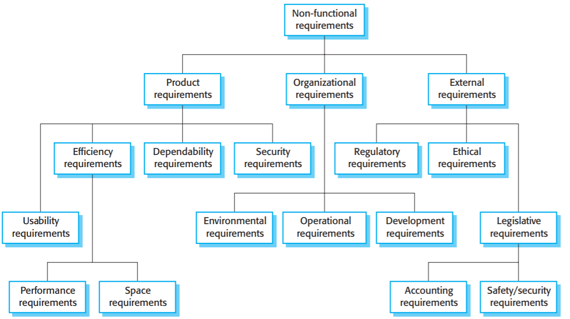
\includegraphics[scale=0.7]{non-functional_requirements.png}
    \end{center}

    Some problems are: stakeholder propose non-functional requirements as goals, it is 
    impossible to objectively verify the goal as been met so try to write them 
    quantitatively.

    \subsection*{Requirements Validation}

    \begin{itemize}
        \item 
        Demonstrates that the requirements define the system that the customer really wants
        \item
        Fixing requirement errors may cost a lot if it has to be done after the product is delivered
        \item
        What to check for:
        \begin{itemize}
            \item 
            Validity
            Requirements reflect the real needs of the system users
            \item
            Consistency
            No requirement contradictions
            \item
            Completeness
            Requirements define all functions and constraints intended by the system user
            \item
            Realism
            Requirements can be implemented within the proposed budget and schedule
            \item
            Verifiability
            System requirements are written in such a way that they can be verified after implementation
        \end{itemize}
    \end{itemize}

    Validation techniques:
    \begin{itemize}
        \item 
        Requirement reviews
        Systematic manual analysis of the requirements
        Performed by both software engineers and users
        \item
        Prototyping
        Develop an executable model of the system
        \item
        Test-case generation
        Develop tests for requirements to check testability
        If test is difficult or impossible to design, often means the requirement will be hard to implement and should be reconsidered
    \end{itemize}

    \section*{System Architecture}

    \subsection*{Architecture Design}

    \begin{itemize}
        \item Understading how a software system should be organized
        \item Designing the overall structure of the system
    \end{itemize}

    Often represented using simple block diagrams 
    \begin{itemize}
        \item High-level picture of the system structure
        \item Each block represents a component in the system 
        \item Arrows represent data or signals passed from one component to another 
    \end{itemize}

    The advantages: easy to understand. Disadvantages: too informal, doesn't show the type of 
    relationships among components or externally visible properties.

    \begin{center}
        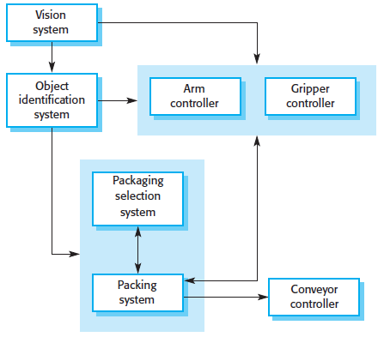
\includegraphics[scale=0.7]{block_diagram.png}
    \end{center}

    \subsection*{4+1 View Model}

    \begin{itemize}
        \item Logical view 
        \begin{itemize}
            \item Key abstractions in the system as objects or object classes
            \item Relate system requirements to objects
        \end{itemize}
        \item Process view 
        \begin{itemize}
            \item How the system is composed of interacting processes
            \item Usingful for making judgement about non-functional requirements 
        \end{itemize}
        \item Development view 
        \begin{itemize}
            \item How the software is decomposed for development 
            \item Useful for software managers and programmers 
        \end{itemize}
        \item Physical view 
        \begin{itemize}
            \item How the system hardware and software components are distributed across 
            the processors in the system 
            \item Useful for system engineers 
        \end{itemize}
        \item +1 link all views through common use cases or scenarios 
    \end{itemize}

    \begin{center}
        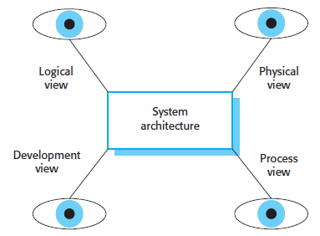
\includegraphics[scale=0.7]{4+1_View_model.png}
    \end{center}

    \subsection*{Architectural Patterns}

    A pattern is a means for representing, sharing, and reusing knowledge; and it may be 
    represented using tabular and graphical descriptions.

    An architectural pattern is a stylized, abstract description of good design practice. 
    It has been tried and tested in diff environments and it should include info about 
    when they are and are not useful and the strengths and weaknesses.

    Examples:
    \begin{itemize}
        \item Model-View-Controller (MVC)
        \item Layered architecture 
        \item repository architecture 
        \item Client-server architecture 
        \item Pipe and filter architecture
    \end{itemize}

    \subsection*{Model-View-Controller}

    Often used for web applications and it splits the system into three different 
    components: Model - stores and manages data; View - GUI; Controller - 
    converts input from the View into demands to retrieve or update data from the 
    Model and passes info from Model to the View.

    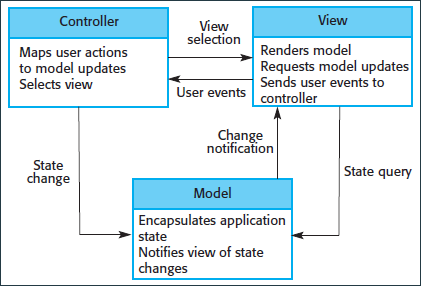
\includegraphics[scale=0.7]{model_view_controller.png}
    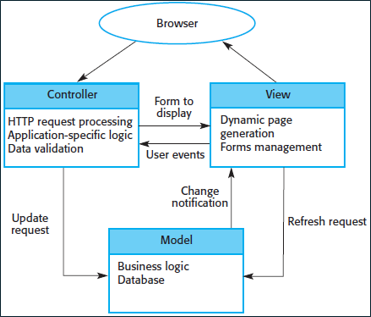
\includegraphics[scale=0.7]{model_view_controller-webbrowser.png}
    \begin{center}
        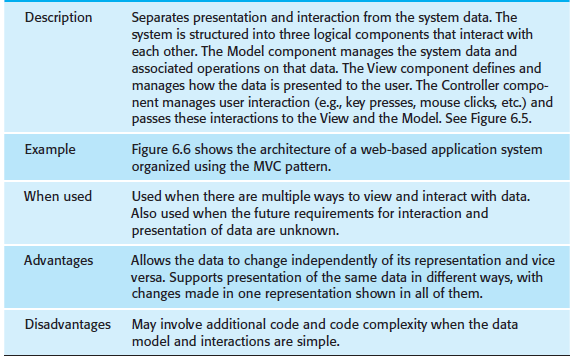
\includegraphics[scale=0.7]{model_view_controller-desc.png}
    \end{center}

    \subsection*{Layered Architecture}    

    Used to model the interfacing of the subsystems and it supports incremental dev 
    of subsystems in diff layers. When a layer interface changes, only the adjacent layers
    are affected. 

    \begin{center}
        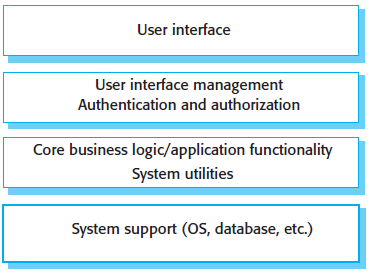
\includegraphics[scale=0.7]{layered_architecture.png}
        The number of layers is arbitrary.

        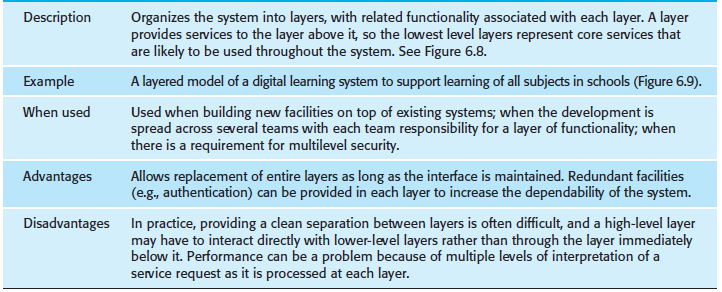
\includegraphics[scale=0.7]{layered_architecture-desc.png}
        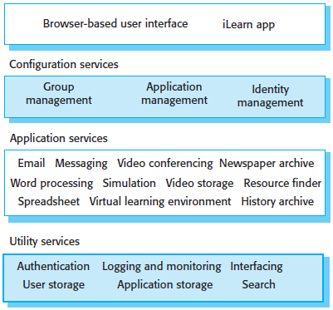
\includegraphics[scale=0.7]{layered_architecture-example.png}
    \end{center}

    \subsection*{Repository Architecture}

    Subsystems must exchange data which can be done by storing datat in central database
    and which can be accessed by all subsystems or each subsystem maintains its own 
    database and passes data to other subsystems. When large amounts of data need to be 
    shared, the repository model is most commonly used.

    \begin{center}
        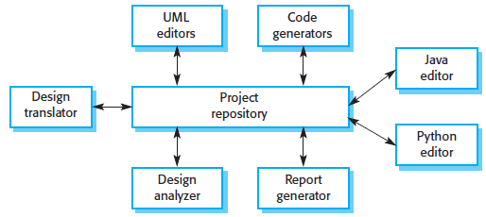
\includegraphics[scale=0.7]{repository_architecture.png}
        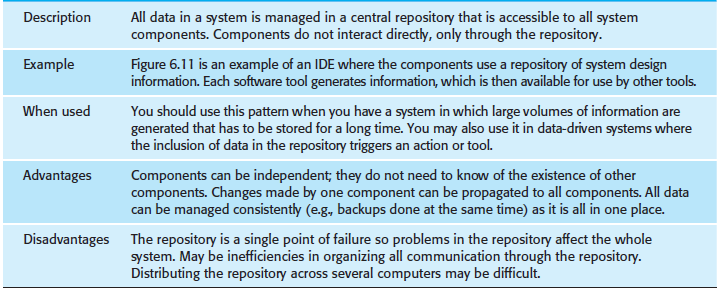
\includegraphics[scale=0.7]{repository_architecture-desc.png}
    \end{center}

    \subsection*{Client-Server Architecture}

    Distributed system model which shows how data and processing is distributed across 
    a range of components. It is a set of stand-alone servers, a set of clients, and a 
    network to connect the two.

    \begin{center}
        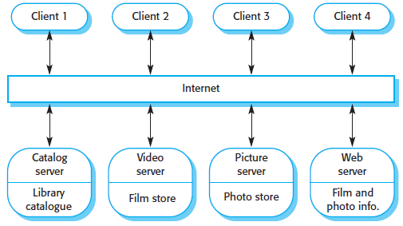
\includegraphics[scale=0.7]{client-server_architecture.png}
        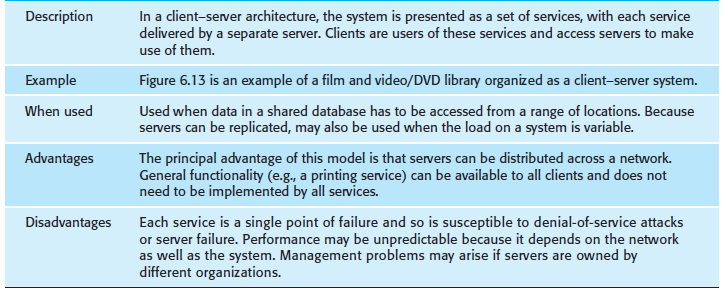
\includegraphics[scale=0.7]{client-server_architecture-desc.png}
    \end{center}

    \subsection*{Pipe and Filter Architecture}

    Data comes into a process, gets transformed and the resulting output is used as the 
    input for the next process. Not a good choice for interactive systems.

    \begin{center}
        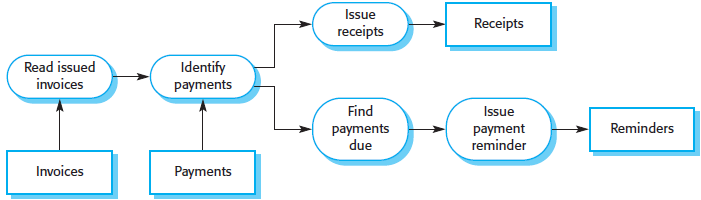
\includegraphics[scale=0.7]{pipe_and_filter_architecture.png}
        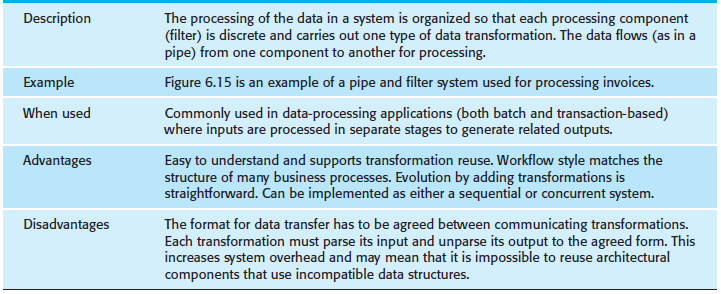
\includegraphics[scale=0.7]{pipe_and_filter_architecture-desc.png}
    \end{center}

    \section*{Design Patterns}
    
    \subsection*{Architecture vs Design}

    Software architecture gives the high-levvel organization of the software and it 
    identifies the main structural components in a system and the relationships between 
    them.

    Sofware design gives the code-level design and it identifies what each class doing, 
    their relationships and scope.

    \subsection*{Design patterns}

    A patter is a description of the problem and the essence of its solution. A design 
    pattern is a way of reusing abstract knowledge about a problem and its solution. 

    It should have High cohesion and low coupling.

    \subsection*{Cohesion}

    Cohesion is the degree of interaction within a module.

    There are 7 levels:
    \begin{itemize}
        \item Functional (best): all essential elements for a single task is in one module 
        \item Sequential 
        \item Communicational 
        \item Procedural 
        \item Temporal 
        \item Logical 
        \item Coincidental (worst): Elements have no conceptual relationship other than the 
        location in the source code. 
    \end{itemize}

    \begin{center}
        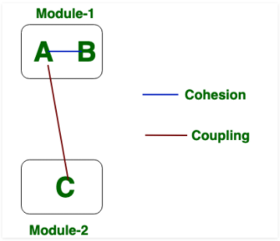
\includegraphics[scale=0.7]{cohesion.png}
    \end{center}

    \subsection*{Coupling}

    Coupling is the degree of interaction between modules.

    There are 5 levels:
    \begin{itemize}
        \item Data (best): modules are independent from each other and communication by 
        only passing data 
        \item Stamp 
        \item Control 
        \item Common 
        \item Content (worst): a module can modify the data of another module.
    \end{itemize}

    \begin{center}
        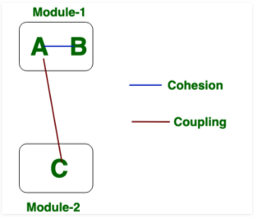
\includegraphics[scale=0.7]{coupling.png}
    \end{center}

    \subsection*{Encapsulation}

    Def: Hides the details from everything; is the process to contain information.

    Implementation: variables of a class are private and functions are public so other 
    classes can get and set the data.

    \begin{center}
        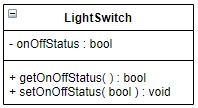
\includegraphics[scale=0.7]{encapsulation.png}
    \end{center}

    \subsection*{Abstraction}

    Def: Shows only what is needed and hides the unwanted info. It is the process to gain 
    info.

    Implementation: Create an abstract class and extend to show more info or add complexity.

    \begin{center}
        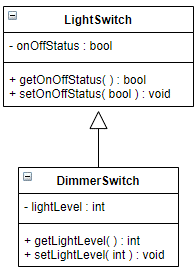
\includegraphics[scale=0.7]{abstraction.png}
    \end{center}

    \subsection*{Design Problems and Patterns}

    To use patterns in your design, you need to recognize that any design problem may have 
    an associated pattern that can be applied.

    There is three catagory: Creational patterns which is focused on creating objects; 
    Structural patterns which setups the relationship between objects; Behavioral patterns 
    which defins how objects interact with each other.

    Examples: 
    \begin{itemize}
        \item Iterator 
        \begin{itemize}
            \item Provide a standard way of accessing the elements in a collection,
            irrespective of how that collection is implemented.
        \end{itemize}
        \item Facade
        \begin{itemize}
            \item Tidy up the interfaces to a number of related objects that have often been 
            developed incrementally
        \end{itemize}
        \item Observer
        \begin{itemize}
            \item Tell several objects that the state of some other objects has changed 
        \end{itemize}
        \item Decorator
        \begin{itemize}
            \item Allow for possibility of extending the functionality of an existing class at 
            run-time
        \end{itemize}
    \end{itemize}

\end{document}